\section{Pengujian Sistem Deteksi Helm Keselamatan Kerja}
\label{sec:system_check}

\par Pada bagian ini akan dipaparkan berbagai macam pengujian terhadap sistem deteksi yang dikembangkan. Seperti yang sebelumnya sudah dijelaskan pada Subab~\ref{sec:perancangansistem}, sistem deteksi helm keselamatan kerja ini akan menjalankan mekanisme alarm berupa suara audio sirine alarm jika dalam frame terdeteksi satu atau lebih kelas "no\_helmet".

\par Pengujian - pengujian sebagian besar dilakukan dengan cara mengambil beberapa sampel gambar dari hasil rekaman sistem di beberapa kondisi berbeda : perbedaan jarak, kecerahan rendah, sudut pandang CCTV, dan percobaan penjalanan di SBC Jetson Nano. Pengujian ini berfokus untuk menjawab pertanyaan "Seberapa akurat sistem menyalakan alarm saat alarm memang dibutuhkan untuk dinyalakan?". Sisi "Positif" akan dilihat dari saat alarm dinyalakan dan "Negatif" saat alarm tidak menyala. 

\subsection{Pengujain Sistem Pada Perbedaan jarak}
\label{subsec:systest_test_dist}

\par Pengujian ini dilakukan dengan pada perbedaan jarak antara kamera dengan objek yang diamati (orang yang memakai atau tidak memakai helm keselamatan kerja). Pengujian dilakukan dengan mengambil beberapa sampel gambar dari rekaman yang menjalankan deteksi pada jarak 1 meter hingga 10 meter.

\begin{table}
    \centering
    \caption{Hasil Pengujain Sistem Pada Perbedaan jarak}
    \label{tb:systest_dist_test}
    \begin{tabular}{|l|l|l|l|l|l|l|} 
    \hline
    Distance & TP & TN & FP & FN & Akurasi    & Jumlah Test  \\ 
    \hline
    1m       & 17 & 61 & 7  & 0  & 0.9176470588 & 85               \\ 
    \hline
    3m       & 20 & 44 & 0  & 2  & 0.9696969697 & 66               \\ 
    \hline
    5m       & 40 & 53 & 0  & 0  & 1            & 93               \\ 
    \hline
    7m       & 32 & 56 & 0  & 0  & 1            & 88               \\ 
    \hline
    10m      & 78 & 32 & 0  & 0  & 1            & 110              \\
    \hline
    \end{tabular}
\end{table}

\par Berdasarkan hasil pengujian yang ditunjukan pada Tabel~\ref{tb:systest_dist_test}, akurasi pada jarak 5 meter hingga 10 meter bernilai 1 karena tidak mengalami kesalahan menyalakan alarm sama sekali dari masing - masing jumlah percobaan seperti yang dapat dilihat pada Gambar~\ref{fig:sys_1-3_meter}. Pada jarak 1 meter dan 3 meter terdapat beberapa \emph{False} dimana pada jarak 1 meter mengalami 7 kali False Positive atau dimana alarm menyala disaat tidak seharusnya menyala dan pada jarak 3 meter terdapat 2 kali False Negative dimana alarm seharusnya menyala tetapi tidak seperti yang dapat dilihat pada Gambar~\ref{fig:sys_5-9_meter}.

\begin{figure} [h]
    \centering
    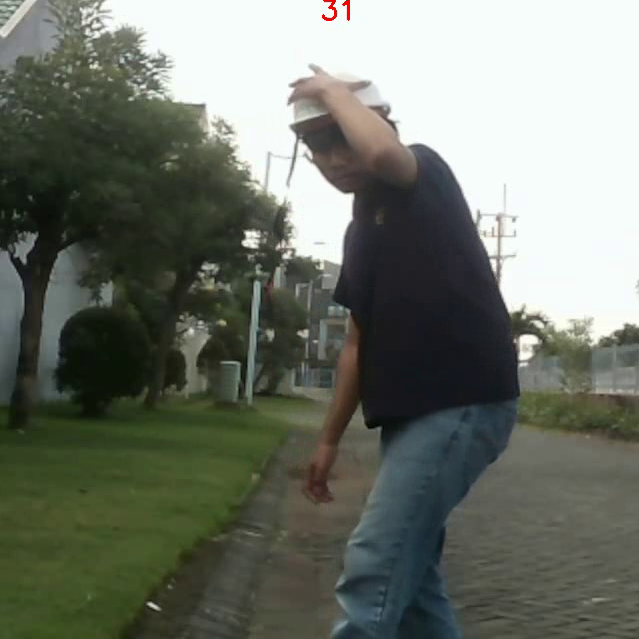
\includegraphics[width=0.3\textwidth]{gambar/sistem_jarak/1-3_jelek/jarak_helmet_white (21).png}
    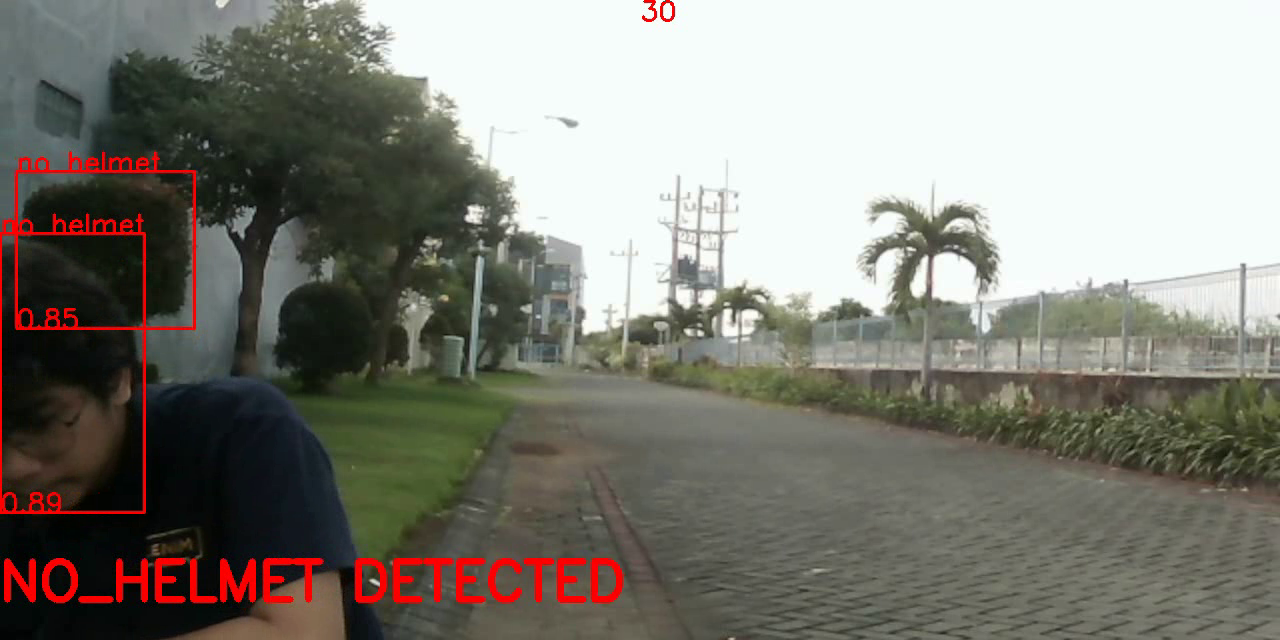
\includegraphics[width=0.3\textwidth]{gambar/sistem_jarak/1-3_jelek/jaraknohelmet (1).png}
    \caption{Deteksi Pada Jarak 1 dan 3 meter}
    \label{fig:sys_1-3_meter}  
\end{figure}

\begin{figure} [h]
    \centering
    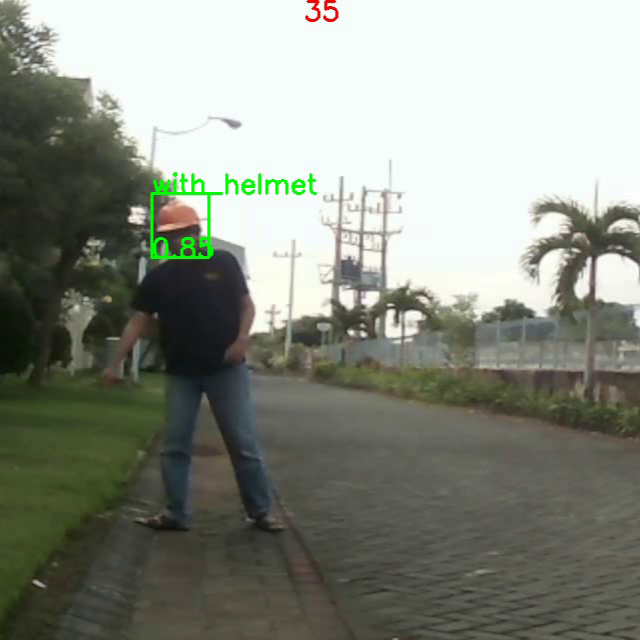
\includegraphics[width=0.3\textwidth]{gambar/sistem_jarak/5-9_bagus/jarak_helmet_orange (67).png}
    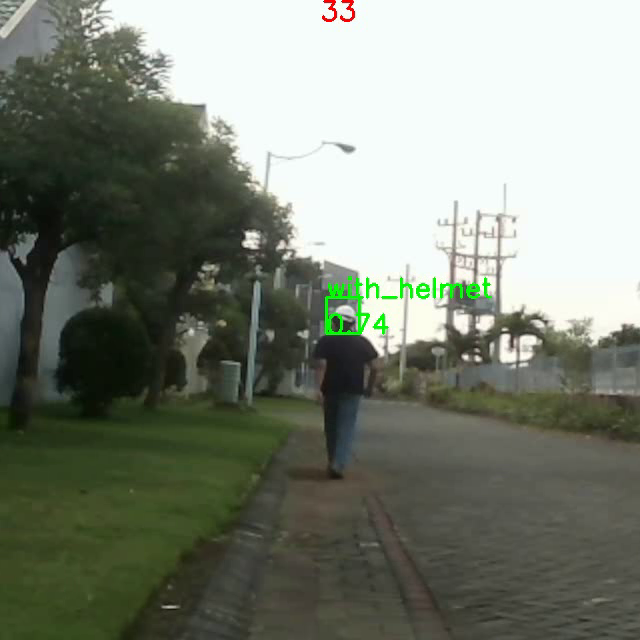
\includegraphics[width=0.3\textwidth]{gambar/sistem_jarak/5-9_bagus/jarak_helmet_white (129).png}
    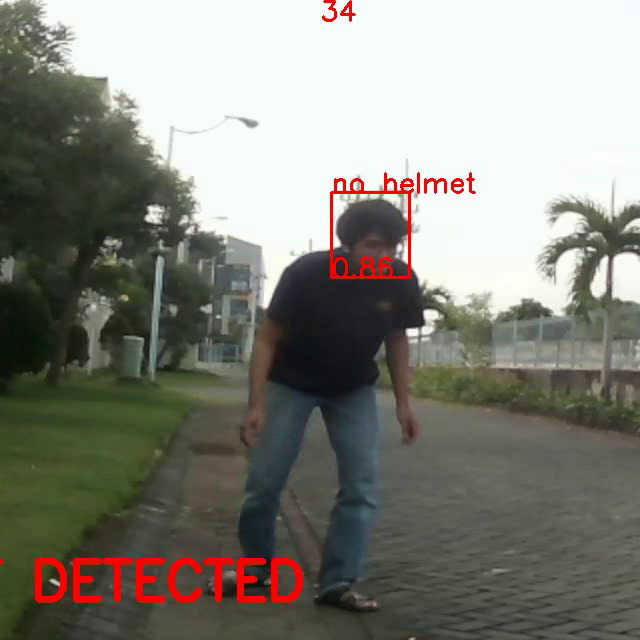
\includegraphics[width=0.3\textwidth]{gambar/sistem_jarak/5-9_bagus/jaraknohelmet (82).png}
    \caption{Deteksi Pada Jarak 5 - 10 meter}
    \label{fig:sys_5-9_meter}  
\end{figure}



\subsection{Pengujian Pada Sudut Pandang CCTV}
\label{subsec:systest_test_cctv}

\par Pengujian ini dilakukan dengan tujuan mengimitasi bagaimana CCTV biasanya dipasang pada suatu \emph{checkpoint} di lokasi konstruksi yang biasanya dipasang dengan sudut 45 derajat. Hasil pengujian ini ditunjukan pada Tabel~\ref{tb:systest_cctv}.


\begin{table}
    \centering
    \caption{Hasil Pengujian Pada Sudut Pandang CCTV}
    \label{tb:systest_cctv}
    \begin{tabular}{|l|l|l|l|l|} 
    \hline
    TP & TN & FP & FN & Akurasi         \\ 
    \hline
    27 & 28 & 0  & 9  & 0.859375         \\ 
    \hline
    \multicolumn{2}{|l|}{55}   & \multicolumn{2}{l|}{9} & 64 tes \\
    \hline
    \end{tabular}
\end{table}

Berdasarkan hasil pengujian tersebut, dari 64 kali pengambilan sampel untuk pengujian, didapati 9 kali \emph{False Negative} dimana terjadi 9 kali kegagalan menyalakan alarm disaat seharusnya menyalakan alarm. Beberapa contoh kegagalan menyalakan alarm atau False Negative ini dicontohkan seperti Gambar~\ref{fig:sys_cctvori_fn}. Tetapi untuk \emph{True Positive} dan \emph{True Negative} lebih banyak terjadi dengan angka 27 dan 28 kali seperti yang ditunjukkan pada Gambar~\ref{fig:sys_cctvori_fn}.

\begin{figure} [h]
    \centering
    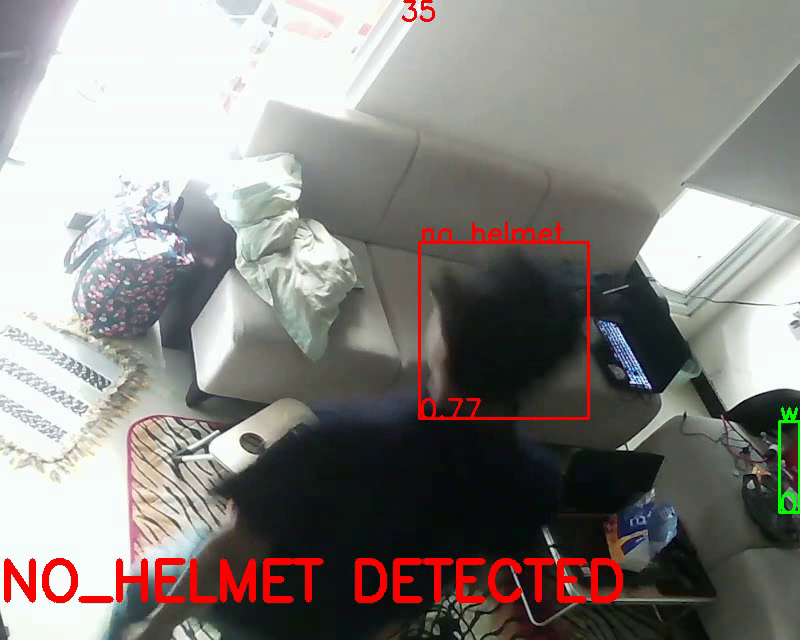
\includegraphics[width=0.3\textwidth]{gambar/sistem_cctvori/betuls/cctv_perspective_pred (7).png}
    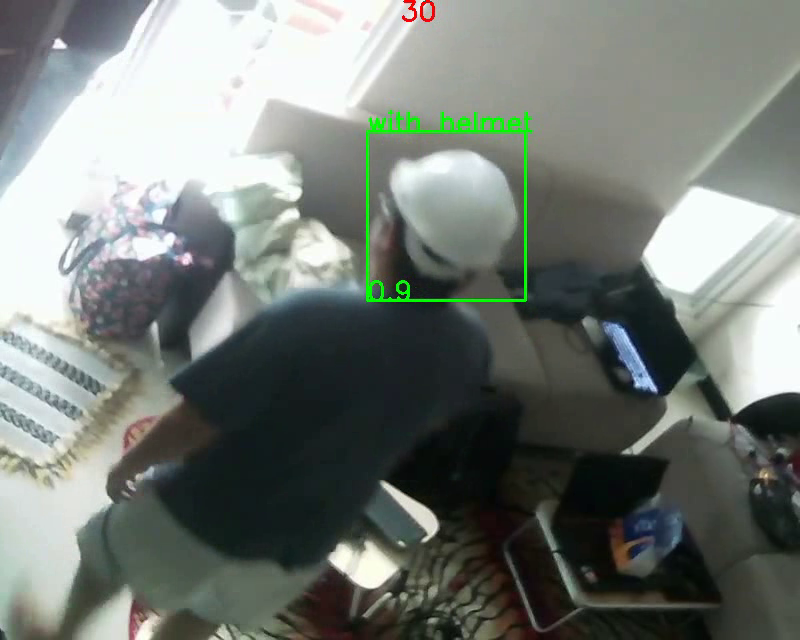
\includegraphics[width=0.3\textwidth]{gambar/sistem_cctvori/betuls/cctv_perspective_pred (11).png}
    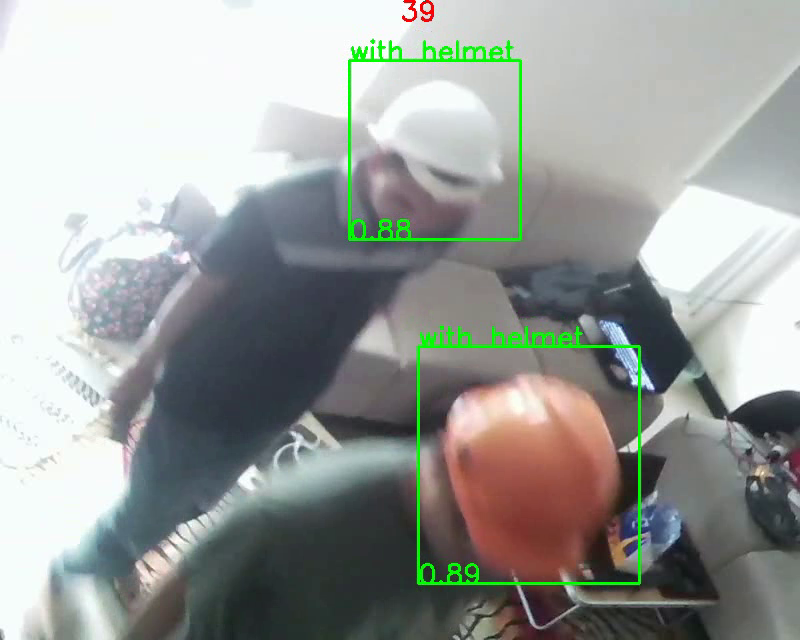
\includegraphics[width=0.3\textwidth]{gambar/sistem_cctvori/betuls/cctv_perspective_pred (53).png}
    \caption{Sistem Deteksi Tepat Pada Sudut 45 Derajat (CCTV)}
    \label{fig:sys_cctvori_true}  
\end{figure}

\begin{figure} [h]
    \centering
    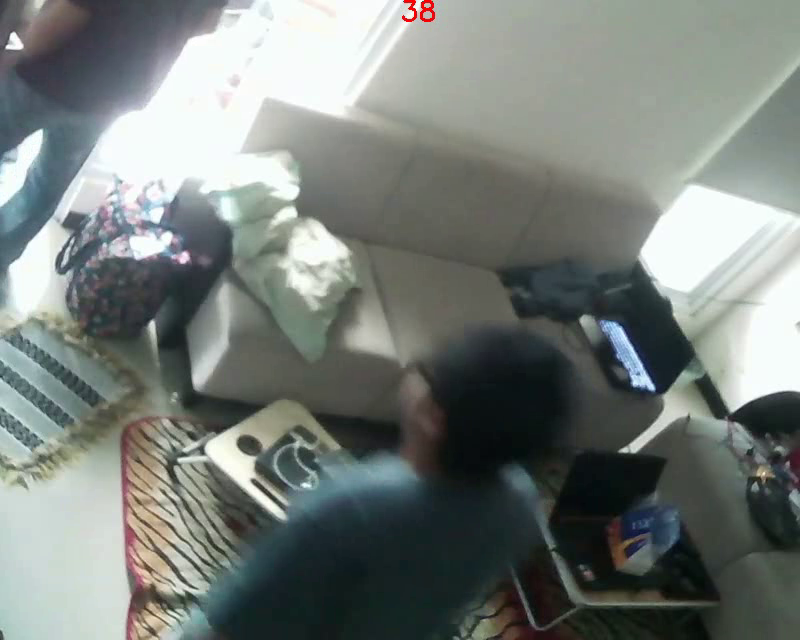
\includegraphics[width=0.3\textwidth]{gambar/sistem_cctvori/falsenegative/cctv_perspective_pred (73).png}
    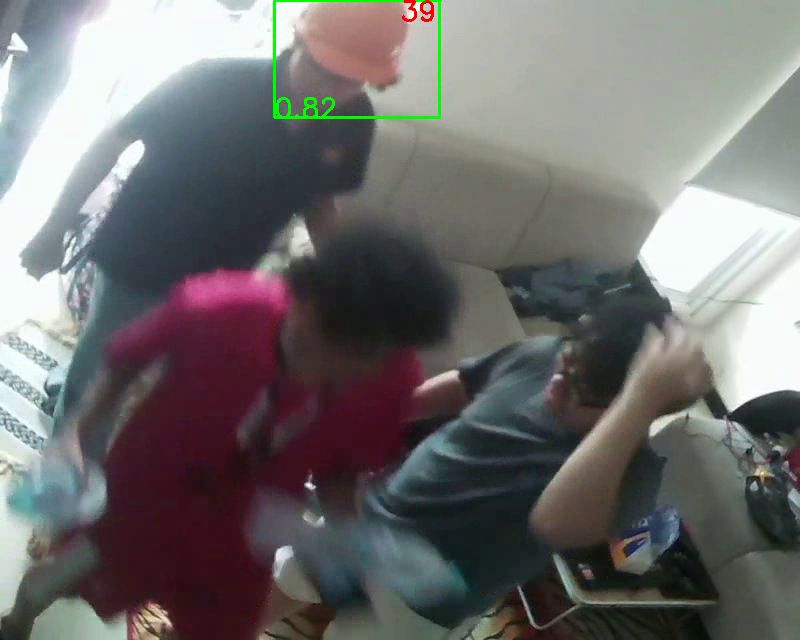
\includegraphics[width=0.3\textwidth]{gambar/sistem_cctvori/falsenegative/cctv_perspective_pred (83).png}
    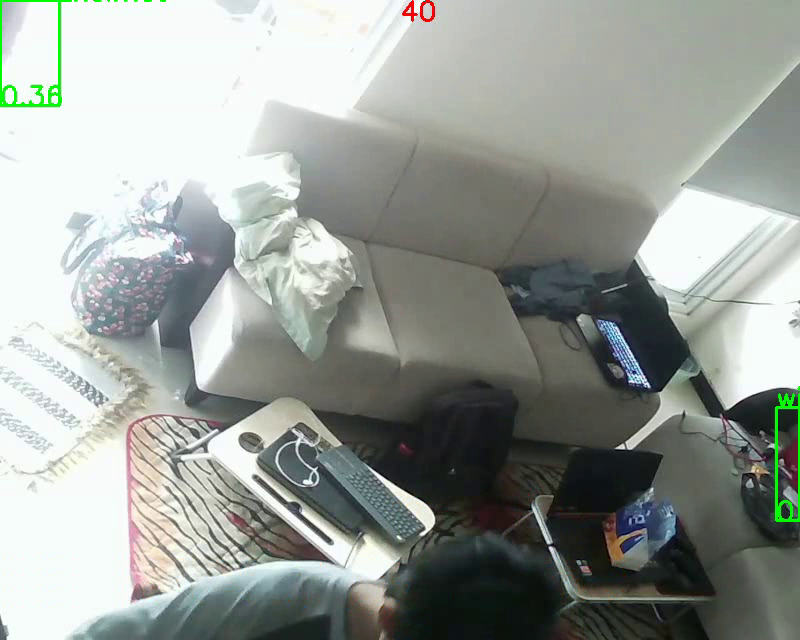
\includegraphics[width=0.3\textwidth]{gambar/sistem_cctvori/falsenegative/cctv_perspective_pred (97).png}
    \caption{Sistem Deteksi \emph{False Negative} Pada Sudut 45 Derajat (CCTV)}
    \label{fig:sys_cctvori_fn}  
\end{figure}


\subsection{Pengujian \emph{Real-Time} Pada Jetson Nano}
\label{subsec:systest_test_jetsonrealtime}

\par Pengujian ini dilakukan dengan memanfaatkan Jetson Nano untuk \emph{deployment} dari sistem deteksi helm keselamatan kerja. Dengan menggunakan camera yang sama dan dipasang dengan sudut yang sama seperti pada Subbab~\ref{subsec:systest_test_cctv} yang lalu dilakukan penjalanan sistem deteksi secara \emph{real-time}. Hasil rekaman penjalanan sistem lalu disimpan dan diambil sejumlah 33 sampel untuk pengujian yang ditunjukan pada Tabel


\begin{table}
    \centering
    \caption{Hasil Pengujian \emph{Real-Time} Pada Jetson Nano}
    \label{tb:systest_jetson}
    \begin{tabular}{|l|l|l|l|l|} 
        \hline
        TP & TN                    & FP & FN                & Akurasi        \\ 
        \hline
        14 & 17                    & 0  & 2                 & 0.9393939394     \\ 
        \hline
        \multicolumn{2}{|l|}{31}   & \multicolumn{2}{l|}{2} & 33 tes  \\
        \hline
    \end{tabular}
\end{table}

\par Pada pengujian ini, ditemukan 2 kali \emph{False Negative} dari 33 kali pengambilan sampel gambar dari rekaman pengujian pada Jetson Nano. Selebihnya 31 pengujian didapati tepat. Lalu didapatkan akurasi pada pengujian ini yaitu 0.94. Beberapa hasil deteksi yang tepat ditunjukkan pada Gambar~\ref{fig:sys_cctvori_fn}.

\subsection{Pengujian Sistem Pada Keadaan Rendah Cahaya (Sore)}
\label{subsec:systest_test_lowilu_sore}

\par Pengujian ini juga dilakukan pada waktu senja ketika penerangan cukup rendah, dan langit masih terang. Hasil pengujian dapat dilihat pada Tabel~\ref{tb:systest_lowillum_dusk}. Untuk pengujian ini terdapat 75 sampel pengujian.

\begin{table}
    \centering
    \caption{Hasil Pengujian Sistem Pada Keadaan Rendah Cahaya (Sore)}
    \label{tb:systest_lowillum_dusk}
    \begin{tabular}{|l|l|l|l|l|} 
        \hline
        TP & TN                    & FP & FN                & Akurasi         \\ 
        \hline
        45 & 25                    & 0  & 5                 & 0.9333333333    \\ 
        \hline
        \multicolumn{2}{|l|}{31}   & \multicolumn{2}{l|}{2} & 70 tes \\
        \hline
    \end{tabular}
\end{table}

\par Pada pengujian dengan tingkat kecerahan rendah dengan penerangan background minimal ini, diambil 70 sampel pengujian. Dari 70 kali pengambil sampel tersebut, didapati 5 kali \emph{False Negative} yang lalu didapati nilai akurasi 0,93. Beberapa hasil pengujian sistem deteksi sistem pada keadaan rendah cahaya pada waktu sore ditunjukkan pada Gambar~\ref{fig:sys_lowilu_sore}.

\begin{figure} [h]
    \centering
    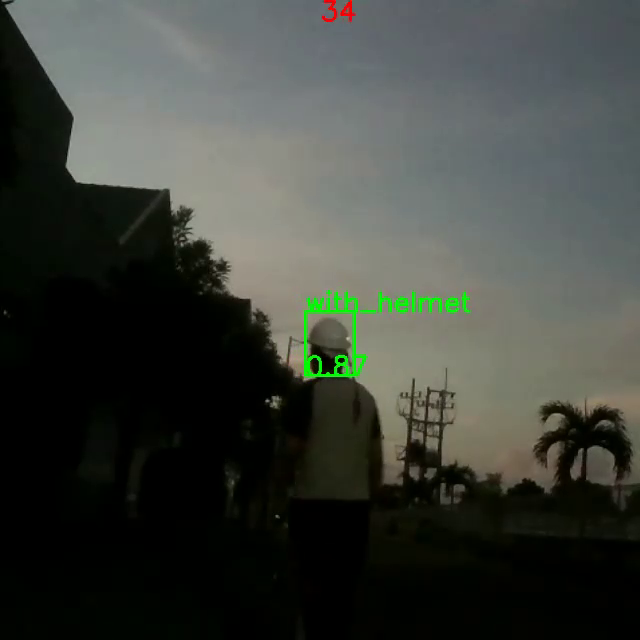
\includegraphics[width=0.3\textwidth]{gambar/sistem-sore/all_alif_5m_pred_Trim (56).png}
    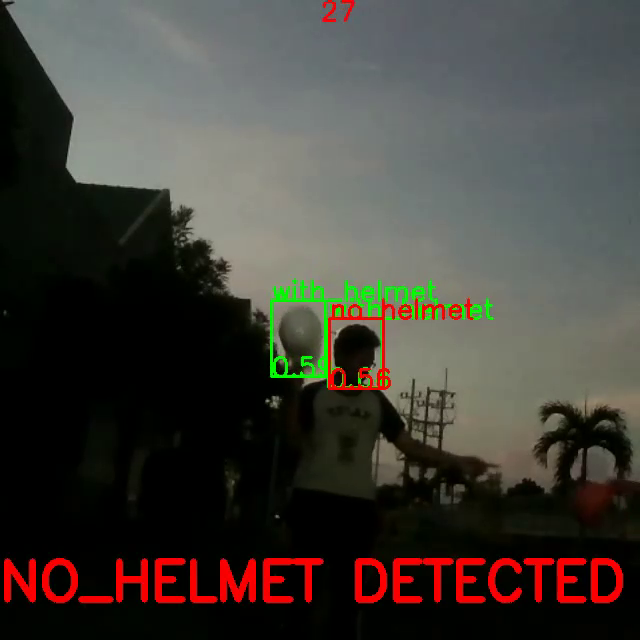
\includegraphics[width=0.3\textwidth]{gambar/sistem-sore/all_alif_5m_pred_Trim (65).png}
    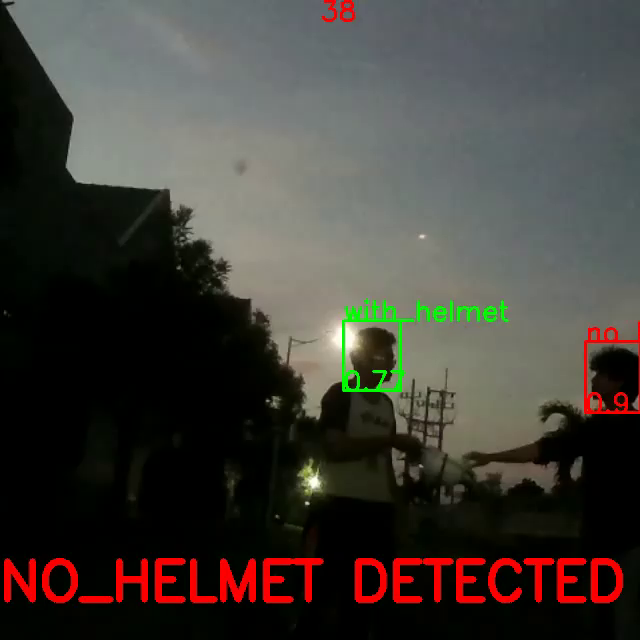
\includegraphics[width=0.3\textwidth]{gambar/sistem-sore/all_alif_5m_pred_Trim (72).png}
    \caption{Contoh Hasil Deteksi Sistem pada Waktu Sore (Pencahayaan Rendah)}
    \label{fig:sys_lowilu_sore}  
\end{figure}

\subsection{Pengujian Sistem Pada Keadaan Rendah Cahaya (Malam)}
\label{subsec:systest_test_lowilu_malam}

\par Tes ini juga dilakukan pada waktu senja ketika penerangan sangat rendah dengan hanya satu sumber cahaya. Hasil pengujian ditunjukkan pada Tabel~\ref{tb:systest_lowillum_dark}. Untuk pengujian ini terdapat 250 sampel pengujian.

\begin{table}
    \centering
    \caption{Hasil Pengujian Sistem Pada Keadaan Rendah Cahaya (Malam)}
    \label{tb:systest_lowillum_dark}
    \begin{tabular}{|l|l|l|l|l|} 
      \hline
      TP & TN                     & FP & FN                 & Akurasi  \\ 
      \hline
      40 & 139                    & 0  & 71                 & 0.716     \\ 
      \hline
      \multicolumn{2}{|l|}{179}   & \multicolumn{2}{l|}{71} &  250 tes    \\
      \hline
    \end{tabular}
\end{table}

\par Pada pengujian dengan tingkat kecerahan sangat rendah pada malam hari dengan penerangan background minimal ini, diambil 250 sampel pengujian. Dari 250 kali pengambil sampel tersebut, didapati 71 kali \emph{False Negative} yang lalu didapati nilai akurasi 0,716. 71 kali kegagalan menyalakan alarm ini disebabkan saat kepala tanpa helm tidak terdetkeis sama sekali yang dimana kebanyakan saat pengujian pada orang yang mengenakan pakaian gelap yang tidak memantulkan cahaya ke wajah yang beberapa dicontohkan pada Gambar~\ref{fig:sys_lowilu_malam_problem}. Nilai akurasi ini sangat jelas menunjukkan terdapat penurunan performa deteksi pada keadaan minim cahaya yang berlebihan. Beberapa contoh hasil deteksi pada waktu malam hari dengan pencahayaan sangat rendah ditunjukkan pada Gambar~\ref{fig:sys_lowilu_malam}.

\begin{figure} [h]
    \centering
    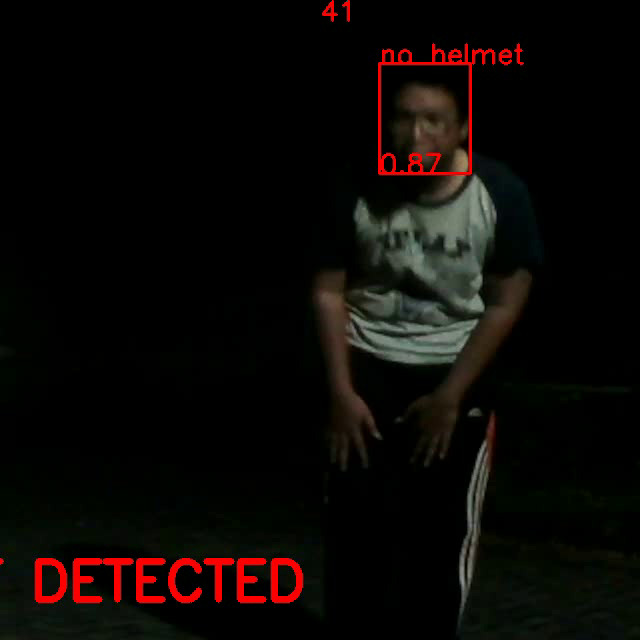
\includegraphics[width=0.3\textwidth]{gambar/sistem_gelap/bagus/gelap_alif_ver2 (1).png}
    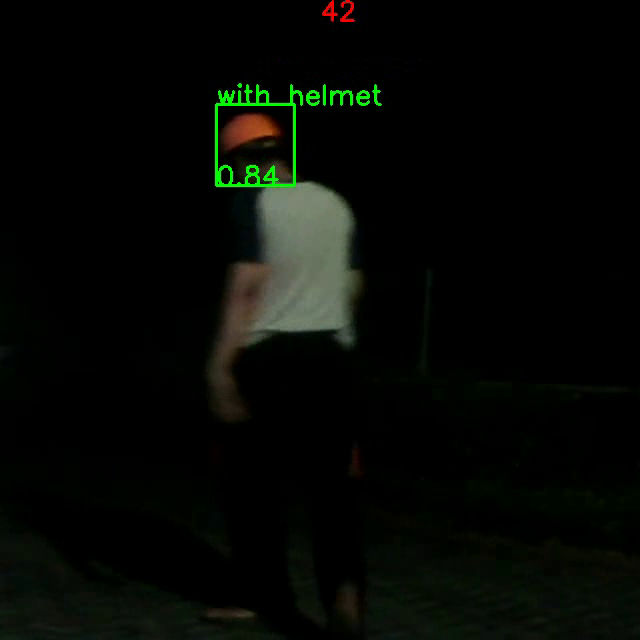
\includegraphics[width=0.3\textwidth]{gambar/sistem_gelap/bagus/gelap_alif_ver2 (54).png}
    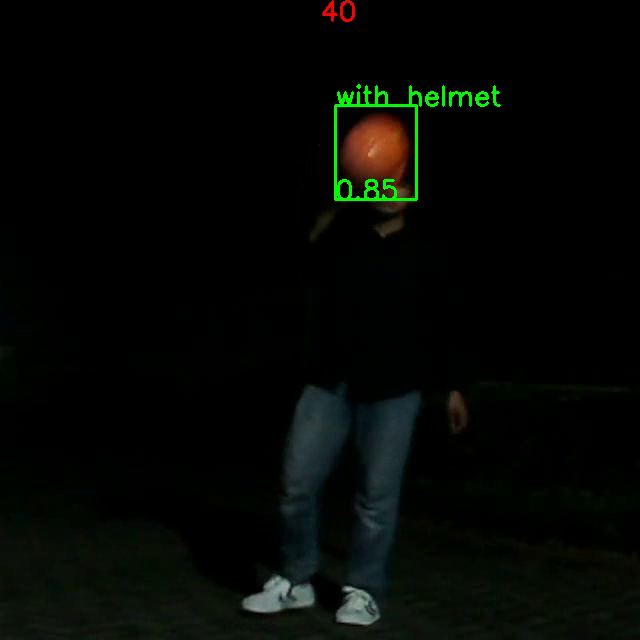
\includegraphics[width=0.3\textwidth]{gambar/sistem_gelap/bagus/gelap_helmika_ver2 (57).png}
    \caption{Contoh Hasil Deteksi Sistem pada Waktu Malam (Pencahayaan Sangat Rendah)}
    \label{fig:sys_lowilu_malam}  
\end{figure}

\begin{figure} [h]
    \centering
    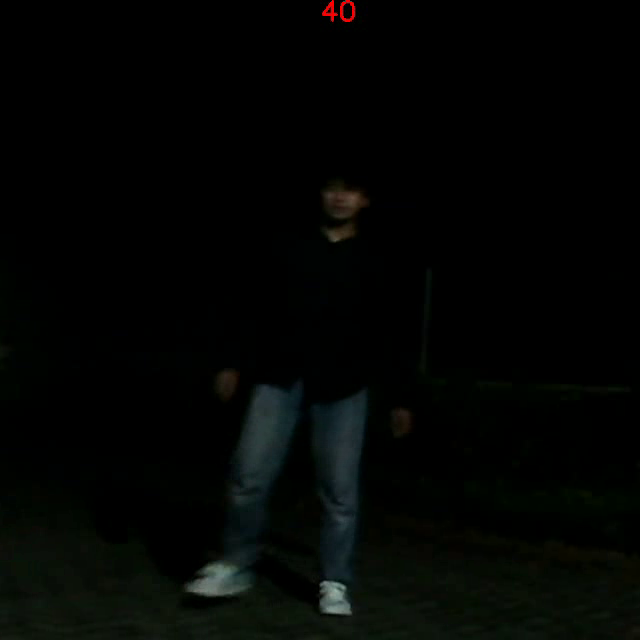
\includegraphics[width=0.3\textwidth]{gambar/sistem_gelap/problem/gelap_helmika_ver2 (19).png}
    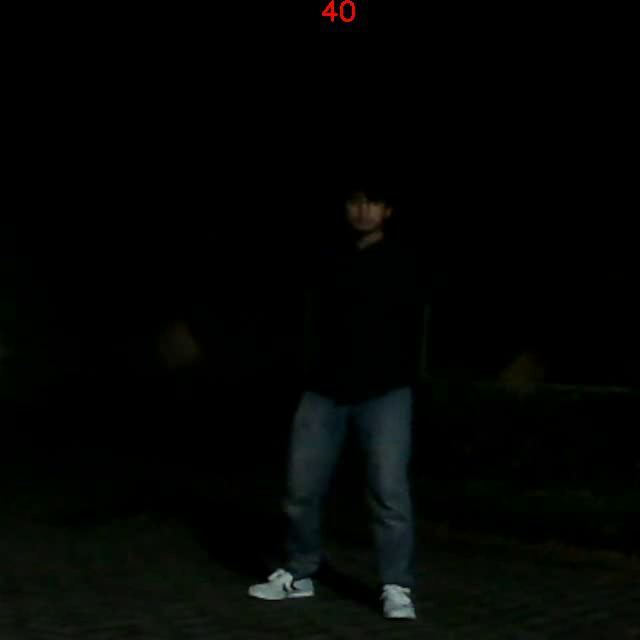
\includegraphics[width=0.3\textwidth]{gambar/sistem_gelap/problem/gelap_helmika_ver2 (26).png}
    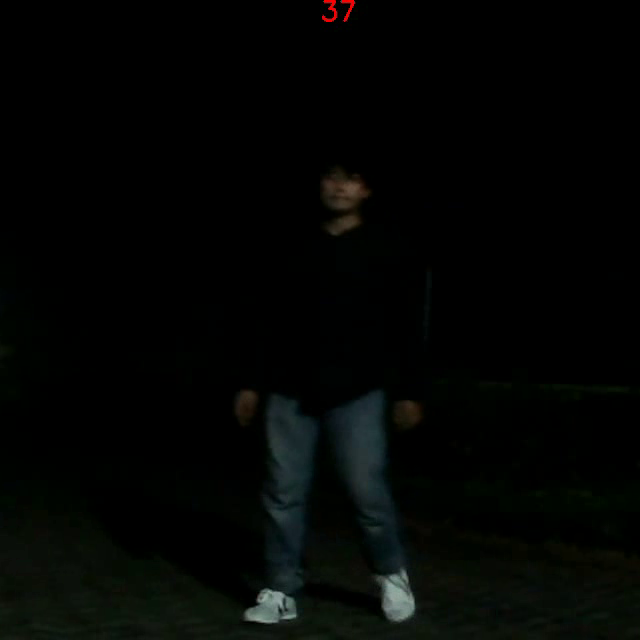
\includegraphics[width=0.3\textwidth]{gambar/sistem_gelap/problem/gelap_helmika_ver2 (33).png}
    \caption{Contoh Hasil Deteksi Sistem pada Waktu Malam (Pencahayaan Sangat Rendah) \emph{False Negative}}
    \label{fig:sys_lowilu_malam_problem}  
\end{figure}